% SC1007 — Chapter 8: Sorting & Asymptotic Analysis
% No \documentclass — included by modules/SC1007/main.tex (book class).
\chapter{Sorting \& Asymptotic Analysis}
\label{ch:graphs-sorting}

\begin{quote}
\emph{``Sorting is the most studied problem in computing.''} --- And the sharpest lens for $O(\cdot)$ reasoning.
\end{quote}

\noindent\textbf{Prerequisites:} Ch.~1--7 (arrays, heaps, recurrences, $O(\cdot)$). This chapter ties SC1007 together: classic sorts, linear-time sorts, lower bounds, and recurrence preview.

\section*{Learning Outcomes}
After this chapter you will be able to:
\begin{enumerate}[label=(L\arabic*)]
    \item implement and analyse quicksort, merge sort, and heap sort;
    \item apply counting sort and radix sort for $O(n)$ sorting under assumptions;
    \item prove the $\Omega(n\log n)$ comparison lower bound via decision trees;
    \item solve recurrences and compare $O(n\log n)$ vs.\ $O(n^{2})$ vs.\ $O(n)$.
\end{enumerate}

% ============================================================
\section{Comparison Sorts: Quick, Merge, Heap}
\label{sec:comparison-sorts}
All comparison sorts must be $\Omega(n\log n)$ worst-case (decision-tree bound, Sec.~\ref{sec:lower-bound}). Three $O(n\log n)$ champions:

\textbf{Merge sort:} divide at mid, recurse, merge $\Theta(n)$. Recurrence $T(n)=2T(n/2)+\Theta(n)\Rightarrow T(n)=\Theta(n\log n)$ worst-case. Stable, not in-place (needs $\Theta(n)$ auxiliary).

\textbf{Heap sort:} build max-heap $O(n)$, repeatedly extract max $O(n\log n)$ in-place, not stable.

\textbf{Quicksort:} partition around pivot $\Theta(n)$, recurse on sides. Average $\Theta(n\log n)$; worst $\Theta(n^{2})$ (bad pivots) but randomised pivot gives expected $\Theta(n\log n)$. In-place, fast in practice.

\begin{figure}[h]
\centering
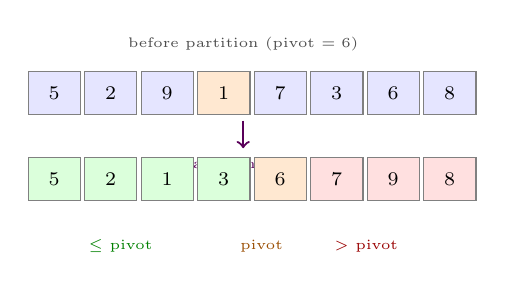
\begin{tikzpicture}[scale=0.78, every node/.style={font=\scriptsize}]
  % Quicksort partition illustration
  \foreach \i/\v/\c in {0/5/blue!10,1/2/blue!10,2/9/blue!10,3/1/orange!18,4/7/blue!10,5/3/blue!10,6/6/blue!10,7/8/blue!10} {
    \draw[fill=\c, draw=black!50] (\i*0.92,0) rectangle ++(0.85,0.70);
    \node at (\i*0.92+0.42,0.35) {\v};
  }
  \node[font=\tiny, gray!60!black] at (3.5,1.15) {before partition (pivot $=6$)};
  \draw[->, thick, violet!70!black] (3.5,-0.1) -- (3.5,-0.55) node[below, font=\tiny] {partition $\Theta(n)$};
  % After
  \foreach \i/\v/\c in {0/5/green!14,1/2/green!14,2/1/green!14,3/3/green!14,4/6/orange!18,5/7/red!12,6/9/red!12,7/8/red!12} {
    \draw[fill=\c, draw=black!50] (\i*0.92,-1.4) rectangle ++(0.85,0.70);
    \node at (\i*0.92+0.42,-1.05) {\v};
  }
  \node[font=\tiny, green!50!black] at (1.5,-2.15) {$\le$ pivot};
  \node[font=\tiny, red!60!black] at (5.5,-2.15) {$>$ pivot};
  \node[font=\tiny, orange!60!black] at (3.8,-2.15) {pivot};
\end{tikzpicture}
\caption{Quicksort partition: pivot $6$ moves to final position; left $\le$ pivot, right $>$ pivot. Recurse on both sides.}
\label{fig:quicksort-partition}
\end{figure}

\begin{lstlisting}[language=Python]
# Quicksort -- Lomuto partition, randomised pivot
import random
def partition(a, lo, hi):
    pivot = a[hi]
    i = lo
    for j in range(lo, hi):
        if a[j] <= pivot:
            a[i], a[j] = a[j], a[i]; i += 1
    a[i], a[hi] = a[hi], a[i]
    return i

def quicksort(a, lo=0, hi=None):
    if hi is None: hi = len(a)-1
    if lo < hi:
        # random pivot for expected O(n log n)
        r = random.randint(lo, hi); a[r], a[hi] = a[hi], a[r]
        p = partition(a, lo, hi)
        quicksort(a, lo, p-1); quicksort(a, p+1, hi)
\end{lstlisting}

\begin{lstlisting}[language=Python]
# Merge sort -- stable, O(n log n) worst-case
def merge(a, lo, mid, hi, tmp):
    i, j, k = lo, mid+1, lo
    while i <= mid and j <= hi:
        if a[i] <= a[j]: tmp[k]=a[i]; i+=1
        else: tmp[k]=a[j]; j+=1
        k+=1
    while i <= mid: tmp[k]=a[i]; i+=1; k+=1
    while j <= hi: tmp[k]=a[j]; j+=1; k+=1
    a[lo:hi+1]=tmp[lo:hi+1]

def mergesort(a, lo=0, hi=None, tmp=None):
    if hi is None: hi=len(a)-1; tmp=[0]*len(a)
    if lo < hi:
        mid=(lo+hi)//2
        mergesort(a,lo,mid,tmp); mergesort(a,mid+1,hi,tmp)
        merge(a,lo,mid,hi,tmp)
\end{lstlisting}

% ============================================================
\section{Linear-Time Sorts}
\label{sec:linear-sorts}
When keys have structure, we beat $n\log n$.

\textbf{Counting sort:} for integers in $[0,k]$, count frequencies, prefix sums give positions. Time $\Theta(n+k)$, space $\Theta(k)$. Stable.

\textbf{Radix sort:} sort by digit from LSD to MSD using stable counting sort per digit. For $d$ digits base $b$: $O(d(n+b))$.

\begin{figure}[h]
\centering
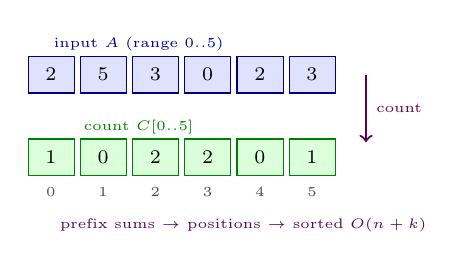
\begin{tikzpicture}[scale=0.78, every node/.style={font=\scriptsize}]
  % Counting sort schematic
  \node[font=\tiny, blue!60!black] at (1.8,2.2) {input $A$ (range $0..5$)};
  \foreach \i/\v in {0/2,1/5,2/3,3/0,4/2,5/3} {
    \draw[fill=blue!12, draw=blue!50!black] (\i*0.85,1.4) rectangle ++(0.75,0.60);
    \node at (\i*0.85+0.37,1.7) {\v};
  }
  \node[font=\tiny, green!50!black] at (1.8,0.85) {count $C[0..5]$};
  \foreach \i/\v in {0/1,1/0,2/2,3/2,4/0,5/1} {
    \draw[fill=green!14, draw=green!50!black] (\i*0.85,0.05) rectangle ++(0.75,0.60);
    \node at (\i*0.85+0.37,0.35) {\v};
    \node[font=\tiny, gray!60!black] at (\i*0.85+0.37,-0.22) {\i};
  }
  \draw[->, thick, violet!70!black] (5.5,1.7) -- (5.5,0.6) node[midway, right, font=\tiny] {count};
  \node[font=\tiny, violet!70!black] at (3.5,-0.75) {prefix sums $\to$ positions $\to$ sorted $O(n+k)$};
\end{tikzpicture}
\caption{Counting sort: histogram $C$ then prefix sums place each element directly. Radix sort repeats this per digit.}
\label{fig:counting-sort}
\end{figure}

\begin{lstlisting}[language=Python]
# Counting sort -- O(n+k), stable
def counting_sort(a, k):
    c = [0]*(k+1)
    for x in a: c[x] += 1
    for i in range(1, k+1): c[i] += c[i-1]
    out = [0]*len(a)
    for x in reversed(a):  # reverse for stability
        c[x]-=1; out[c[x]]=x
    return out

# Radix sort -- LSD first, stable per digit
def radix_sort(a, base=10):
    maxv = max(a) if a else 0
    exp = 1
    while maxv // exp > 0:
        # counting sort by digit (exp place)
        buckets = [[] for _ in range(base)]
        for x in a: buckets[(x//exp) % base].append(x)
        a = [x for b in buckets for x in b]
        exp *= base
    return a
\end{lstlisting}

% ============================================================
\section{Lower Bound \& Analysis}
\label{sec:lower-bound}
\begin{theorem}[Comparison lower bound]
Any comparison sort needs $\Omega(n\log n)$ comparisons worst-case.
\end{theorem}
\begin{proof}[Sketch]
Decision tree has $n!$ leaves (one per permutation). Binary tree with $L$ leaves has height $\ge\lceil\log_{2}L\rceil$. So height $\ge\log_{2}(n!)=\Theta(n\log n)$ by Stirling.
\end{proof}

\begin{figure}[h]
\centering
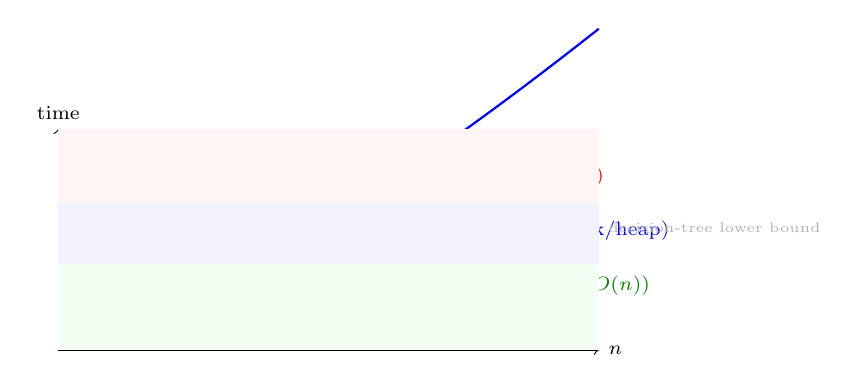
\begin{tikzpicture}[scale=0.78, every node/.style={font=\scriptsize}]
  \draw[->] (0,0) -- (8.8,0) node[right] {$n$};
  \draw[->] (0,0) -- (0,3.6) node[above] {time};
  \draw[red, thick] plot[domain=0.3:8.8, smooth] (\x,{0.25+0.32*\x});
  \node[red] at (7.8,2.85) {$n^{2}$ (insertion)};
  \draw[blue, thick] plot[domain=0.3:8.8, smooth] (\x,{0.25+0.55*\x*ln(\x+1)/ln(2)/3.2});
  \node[blue] at (7.8,1.95) {$n\log n$ (merge/quick/heap)};
  \draw[green!50!black, thick] plot[domain=0.3:8.8, smooth] (\x,{0.25+0.32*\x/2.5});
  \node[green!50!black] at (7.8,1.05) {$n$ (counting, $k=O(n)$)};
  \draw[dashed, gray!60] (0,2.0) -- (8.8,2.0) node[right, font=\tiny] {decision-tree lower bound};
  \fill[green!5] (0,0) rectangle (8.8,1.4);
  \fill[blue!5] (0,1.4) rectangle (8.8,2.4);
  \fill[red!4] (0,2.4) rectangle (8.8,3.6);
\end{tikzpicture}
\caption{Sorting landscape: comparison sorts cannot beat $n\log n$; counting/radix break the bound by using key structure.}
\label{fig:sorting-landscape}
\end{figure}

\textbf{Recurrence preview:} merge sort $T(n)=2T(n/2)+\Theta(n)=\Theta(n\log n)$; quicksort average $T(n)=T(k)+T(n-k-1)+\Theta(n)$ with $k\sim\text{Uniform}$ gives $\Theta(n\log n)$ expected.

% ============================================================

% --- Additional: Stability and hybrid sorts ---
\section{Stability, Hybrids \& Recurrence Details}
\label{sec:stability-hybrids}
\textbf{Stability.} A sort is \emph{stable} if equal keys retain input order. Merge and counting/radix are stable; heap and quicksort (as usually implemented) are not. Stability matters when sorting by multiple keys.

\textbf{Introsort} (STL \texttt{sort}) runs quicksort but switches to heapsort when recursion depth exceeds $2\log n$, guaranteeing $O(n\log n)$ worst-case while keeping quicksort's speed. Small subarrays ($<16$) use insertion sort.

\textbf{Recurrence bridge to SC2001.} Merge sort gives $T(n)=2T(n/2)+\Theta(n)$. Master theorem (SC2001 Ch.~3) yields $\Theta(n\log n)$. Quicksort average case uses indicator variables: expected comparisons $=2\sum_{i<j}1/(j-i+1)=\Theta(n\log n)$.

\begin{lstlisting}[language=Python]
# Introsort sketch -- depth-limited quicksort
import heapq
def introsort(a, lo, hi, depth_limit):
    if hi - lo < 16:
        insertion_sort(a, lo, hi); return
    if depth_limit == 0:
        heapsort_range(a, lo, hi); return
    p = partition(a, lo, hi)
    introsort(a, lo, p-1, depth_limit-1)
    introsort(a, p+1, hi, depth_limit-1)
\end{lstlisting}

\section{Chapter Notes}
CLRS Ch.~2, 6--8, Weiss Ch.~7. Quicksort is usually fastest in practice despite worst case; introsort (STL \texttt{sort}) switches to heapsort when recursion deepens.

% ============================================================
\section{Exercises}
\label{sec:ch08-exercises}
\begin{enumerate}[label=E8.\arabic*, leftmargin=*, itemsep=0.7em]
    \item \textbf{Quicksort trace.} Sort $[5,2,9,1,7,3,6,8]$ with quicksort, pivot $=$ last element. Show partitions and recursion tree. Count comparisons.
    \item \textbf{Merge analysis.} Prove $T(n)=2T(n/2)+n=\Theta(n\log n)$ by recursion tree. Is merge sort stable? Is it in-place? Justify.
    \item \textbf{Counting sort.} Sort $[2,5,3,0,2,3]$ with counting sort ($k=5$). Show $C$, prefix sums, and output construction. Why does iterating reversed preserve stability?
    \item \textbf{Lower bound.} Prove $\log_{2}(n!)=\Theta(n\log n)$ using Stirling or integral bounds. Explain why counting sort does not violate the comparison lower bound.
    \item \textbf{Hybrids.} Describe introsort (quicksort $\to$ heapsort fallback + insertion sort for small $n$). Why does STL use it? Analyse its $O(n\log n)$ worst-case guarantee.
\end{enumerate}
% End of Chapter 8
